
\documentclass[pdf, unicode, 12pt, a4paper,oneside,fleqn]{article}
\usepackage{graphicx}
\graphicspath{{img/}}
\usepackage{log-style}
\begin{document}

\begin{titlepage}
    \begin{center}
        \bfseries

        {\Large Московский авиационный институт\\ (национальный исследовательский университет)}
        
        \vspace{48pt}
        
        {\large Факультет информационных технологий и прикладной математики}
        
        \vspace{48pt}
        
        Лабораторная работа \textnumero 4 по курсу \enquote{Операционные системы}

        \vspace{48pt}

        Освоение принципов работы с файловыми системами. 
        
        Обеспечение обмена данных между процессами посредством технологии <<File mapping>>.
    \end{center}
    
    \vspace{140pt}
    
    \begin{flushright}
    \begin{tabular}{rl}
    Студент: & П.\,Ф. Гришин \\
    Преподаватель: & Е.\,С. Миронов \\
    Группа: & М8О-201Б-21 \\
    Вариант: & 16 \\
    Дата: & \\
    Оценка: & \\
    Подпись: & \\
    \end{tabular}
    \end{flushright}
    
    \vfill
    
    \begin{center}
    \bfseries
    Москва, \the\year
    \end{center}
\end{titlepage}
    
\pagebreak

\section{Постановка задачи}

Составить и отладить программу на языке Си, осуществляющую работу с процессами
и взаимодействие между ними в одной из двух операционных систем. В результате
работы программа (основной процесс) должен создать для решение задачи один или
несколько дочерних процессов. Взаимодействие между процессами осуществляется
через системные сигналы/события и/или каналы (pipe).
Необходимо обрабатывать системные ошибки, которые могут возникнуть в резуль-
тате работы.
Родительский процесс создает дочерний процесс. Первой строкой пользователь в
консоль родительского процесса вводит имя файла, которое будет использовано для
открытия File с таким именем на запись. Перенаправление стандартных потоков
ввода-вывода показано на картинке выше. Родительский и дочерний процесс долж-
ны быть представлены разными программами. Родительский процесс принимает от
пользователя строки произвольной длины и пересылает их в pipe1.
Процесс child проверяет строки на валидность правилу. Если строка соответствует
правилу, то она выводится в стандартный поток вывода дочернего процесса, иначе в
pipe2 выводится информация об ошибке. Родительский процесс полученные от child
ошибки выводит в стандартный поток вывода.
Правило проверки: строка должна оканчиваться на «.» или «;»

\begin{figure}[htp]
    \centering
    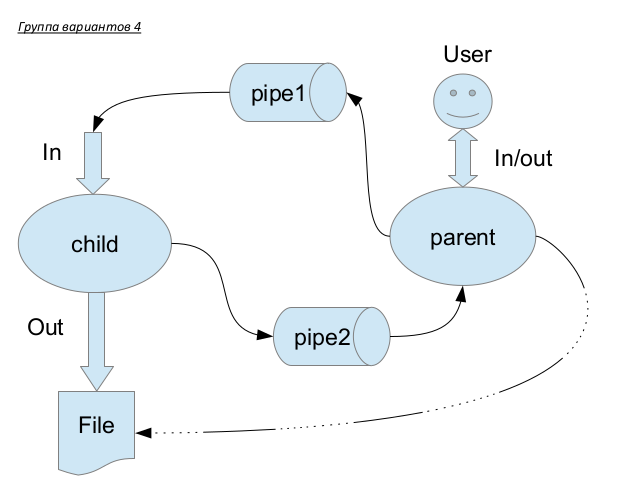
\includegraphics[width=11cm]{os2.png}
    \caption{Структура программы}
    \label{fig:os2}
\end{figure}

\section{Сведения о программе}

Программа написанна на Си в Unix подобной операционной системе на базе ядра
Linux. В программе создается дочерний процесс, в который перенаправляются дан-
ные из pipe.

Дочерний прочесс принимает строку чисел и находит их сумму, ответ записывая в
файл. Имя файла задается пользователем
Родительский процесс считывает вводные данные у пользоветеля и пердет их дочер-
нему процессу через pipe.

Программа завершает работу при окончании ввода, то есть нажатии CTRL+D.

\section{Общий метод и алгоритм решения}
Все проверки совершаются через функцию Handle\_error.

При запуске программы прользоваательль может ввести имя файла, который создаст
дочерняя программа.
После запуска создается pipe, два файловых дескриптора для потока ошибок и для
общения между родительским и дочерним процессом.

Родительский процесс просит пользователя ввести имя файла, в котором содержатся
имя выходного файла и данные. После проверки файла на ошибки начинается пе-
редача через файловый дескриптор src\_fd строки. После этого создается дочерний
процесс с помощью \textbf{fork()}. В нем дескриптор потока ввода заменяется на поток вы-
вода из pipe. Таким образом, когда родитель запишет что-то в pipe ребенок сможет
это считать, как будто ввод происходит из консоли. После проверки файла на ошиб-
ки начинается передача через файловый дескриптор src\_fd строки. После замены
дескрипторов вызывается дочерняя прогграмма с помощью \textbf{execl()}. В нее имя фай-
ла передается как параметр при запуске. Далее дочерний процесс обработает строку
и выведет свой вердикт подходит ли данная строка или нет. Если она подходит, то
дочерний процесс даст сигнал родителю, что строка валидна. Иначе - вызовет поток
ошибок (файловый дескриптор error\_fd) и передаст родительскому процессу. В свою
очередь, родитель выведет пользователю сообщение о том, что строка не подходит.

При нажатии CTRL+D пользователь сигнализирует о конце ввода. Родительский
процесс завершает работу, а вместе с ним и дочерний.

\section{Листинг программы}
{\large\textbf{parent.c}}

\begin{lstlisting}[language=C]
 #include "library.h"
 #include "utils.h"

 void ParentRoutine(char* nameF){
    FILE* file = fopen(nameF, "r");
     Handle_error(file == NULL , "open error");

    int src_fd[2];
    int pipe_response = pipe(src_fd);
    Handle_error(pipe_response == -1, "pipe error");

    int err_fd[2];
    pipe_response = pipe(err_fd);
    Handle_error(pipe_response == -1, "pipe error");

    pid_t id = fork();
    Handle_error(id == -1, "fork error");

    if (id == 0){

        char name[64];
        read(src_fd[0], &name, sizeof(name));

        char *src_fd_0, *src_fd_1, *err_fd_0, *err_fd_1;
        asprintf(&src_fd_0, "%d", src_fd[0]);
        asprintf(&src_fd_1, "%d", src_fd[1]);
        asprintf(&err_fd_0, "%d", err_fd[0]);
        asprintf(&err_fd_1, "%d", err_fd[1]);

        execl("child", name, src_fd_0, src_fd_1, err_fd_0, err_fd_1, NULL);

    } else {
        char* parent;
        int parent_pid = getpid();
        printf("[%d] PARENT. ",parent_pid);
        printf("Enter the name of file to write: ");
        char name[256];
        fscanf(file, "%s", name);
        Clean(name);
        printf("%s\n", name);
        write(src_fd[1], &name, sizeof(name));
        bool file_error;
        read(err_fd[0], &file_error, sizeof(bool));
        if (file_error){
            close(src_fd[0]); close(src_fd[1]);
            close(err_fd[0]); close(err_fd[1]);
            Handle_error(true, "file error\n");
        }

        char str[256];
        printf("[%d] PARENT. ",parent_pid);
        printf("Enter string: ");
        while (fscanf(file, "%s", str) != EOF){
            Clean(str);
            printf("%s\n", str);
            write(src_fd[1], &str, sizeof(str));
            bool err;
            read(err_fd[0], &err, sizeof(bool));
            if (err){
                char* err_msg;
                asprintf(&err_msg, "Error: \"%s\" is not valid.\n", str);
                printf("[%d] PARENT. ",parent_pid);
                printf("Error: \"%s\" is not valid.\n", str);
            }
            printf("[%d] PARENT. ",parent_pid);
            printf("Enter string: ");
        }
        write(src_fd[1], "_quit", sizeof(str));

    }
    write(fileno(stdout), "\n", sizeof "\n");
    close(src_fd[0]); close(src_fd[1]);
    close(err_fd[0]); close(err_fd[1]);
    fclose(file);
}
\end{lstlisting}

{\large\textbf{child.c}}

\begin{lstlisting}[language=C]
 #include "library.h"
 #include "utils.h"

int main(int argv, char* argc[]){

    int src_fd[2], err_fd[2];
    src_fd[0] = atoi(argc[1]);
    src_fd[1] = atoi(argc[2]);
    err_fd[0] = atoi(argc[3]);
    err_fd[1] = atoi(argc[4]);

    char* name = argc[0];
    int output_fd = open(name, O_WRONLY | O_CREAT);
    bool file_error = false;
    if (output_fd < 0) file_error = true;
    write(err_fd[1], &file_error, sizeof(bool));
    if (file_error){
        close(src_fd[0]); close(src_fd[1]);
        close(err_fd[0]); close(err_fd[1]);
    }

    char str[256];
    read(src_fd[0], &str, sizeof(str));
    read(src_fd[0], &str, sizeof(str));
    while(strcmp(str, "_quit") != 0){
        bool err;
        int lastIndex = StrLength(str);
        if (StrLength(str)){
            err = false;
            write(output_fd, str, (strlen(str)) * sizeof(char));
            write(output_fd, "\n", 1);
        } else {
            err = true;
        }
        write(err_fd[1], &err, sizeof(bool));
        read(src_fd[0], &str, sizeof(str));
    }
    close(src_fd[0]); close(src_fd[1]);
    close(err_fd[0]); close(err_fd[1]);
}



\end{lstlisting}

\section{Демонстрация работы программы}

\begin{alltt}
gpavel@gpavel-HP-Pavilion-Gaming-Laptop-17-cd1xxx:~/Desktop/OS/lab2$ ./Lab2 
test.txt
[43971] PARENT. Enter the name of file to write: OutputFile.txt
[43971] PARENT. Enter string: FirstTest.
[43971] PARENT. Enter string: False
[43971] PARENT. Error: "False" is not valid.
[43971] PARENT. Enter string: CCCCCCCCCCCCCCCCCCC.
[43971] PARENT. Enter string: End;
[43971] PARENT. Enter string: ...........................a
[43971] PARENT. Error: "...........................a" is not valid.
[43971] PARENT. Enter string: wave...;
[43971] PARENT. Enter string: wrongString
[43971] PARENT. Error: "wrongString" is not valid.

[43971] PARENT. Enter string: 
gpavel@gpavel-HP-Pavilion-Gaming-Laptop-17-cd1xxx:~/Desktop/OS/lab4$ 

\end{alltt}

\pagebreak

\section{Вывод}

Одна из основных задач операционной системы - это управление процессами.
В большинстве случаев она сама создает процессы для себя и при запуске других программ.
Тем не менее бывают случаи, когда необходимо создавать процессы вручную.

В языке Си есть функционал, который позволит нам внутри нашей программы создать
дополнительный, дочерний процесс. Этот процесс будет работать параллельно с родительским.

Для создания дочерних процессов используется функция fork. При этом с помощью ветвлений 
в коде можно отделить код родителя от ребенка. У ребенка при этом можно заменить программу,
испрользуя для этого функцию exec, а обеспечить связь с помощью pipe.

Подобный функционал есть во многих языках программирования, так как большинство современных программ состаят более, чем из одного процесса.

\end{document}

